\section*{Radiation Balance Between Parallel Plates}
Assignment is completed by Mikkel Jaedicke (mijae12) \& Anders Bæk (anbae12)

Equation \ref{eq:1} is known to be true for Saturn's double moon. Where $\left[ \begin{matrix} x_{ i } \\ y_{ i } \end{matrix} \right]$ denotes moon i's position in a cartesian coordinate system with Saturn as origo. 

\begin{equation}
\begin{align*}
m_{ 1 }\frac { { d }^{ 2 } }{ { dt }^{ 2 } } \left[ \begin{matrix} x_{ 1 } \\ y_{ 1 } \end{matrix} \right] &=-\frac { m_{ 1 }\cdot M\cdot g }{ { r }^{ 3 }_{ 1 } } \left[ \begin{matrix} x_{ 1 } \\ y_{ 1 } \end{matrix} \right] +\frac { m_{ 1 }\cdot m_2\cdot g }{ { r }^{ 3 }_{ 12 } } \left[ \begin{matrix} x_{ 2 }-x_{ 1 } \\ y_{ 2 }-y_{ 1 } \end{matrix} \right] \\
m_{ 2 }\frac { { d }^{ 2 } }{ { dt }^{ 2 } } \left[ \begin{matrix} x_{ 2 } \\ y_{ 2 } \end{matrix} \right] &=-\frac { m_{ 2 }\cdot M\cdot g }{ { r }^{ 3 }_{ 2 } } \left[ \begin{matrix} x_{ 2 } \\ y_{ 2 } \end{matrix} \right] -\frac { m_{ 1 }\cdot m_{ 2 }\cdot g }{ { r }^{ 3 }_{ 12 } } \left[ \begin{matrix} x_{ 2 }-x_{ 1 } \\ y_{ 2 }-y_{ 1 } \end{matrix} \right] 
\end{align*}
\label{eq:1}
\end{equation}
where: \( m_1 = m_2 =9.20 \cdot 10^{18} \) [kg], \( M = 5.68  \cdot 10^{26} \) [kg], \( g = 4.98 \cdot 10^{-10} \left[ \frac { \text{km}^3 }{ \text{kg} \cdot \text{døgn} }  \right] \).

The initial values in equation \ref{eq:2} are also known to be true.
\begin{equation}
\begin{align*}
\left[ \begin{matrix} x_{ 1 } \\ y_{ 1 } \end{matrix} \right] &=\left[ \begin{matrix} 0 \\ 152870 \end{matrix} \right] ,\;\;\; 
\frac { d }{ dt } \left[ \begin{matrix} x_{ 1 } \\ y_{ 1 } \end{matrix} \right] =\left[ \begin{matrix} -1360278.1 \\ 0 \end{matrix} \right]  \\
\left[ \begin{matrix} x_{ 2 } \\ y_{ 2 } \end{matrix} \right] &=\left[ \begin{matrix} 0 \\ -153130 \end{matrix} \right] ,\; \;\;
\frac { d }{ dt } \left[ \begin{matrix} x_{ 2 } \\ y_{ 2 } \end{matrix} \right] =\left[ \begin{matrix} 1359122.8 \\ 0 \end{matrix} \right] 
\end{align*}
\label{eq:2}
\end{equation}

\noindent\makebox[\linewidth]{\rule{\textwidth}{0.4pt}}

\section{Calculations}
Equation \ref{eq:3} is obtained by dividing equation \ref{eq:1} by $m_i$.

\begin{equation}
\begin{align*}
\frac { { d }^{ 2 } }{ { dt }^{ 2 } } \left[ \begin{matrix} x_{ 1 } \\ y_{ 1 } \end{matrix} \right] =-\frac { M\cdot g }{ { r }^{ 3 }_{ 1 } } \left[ \begin{matrix} x_{ 1 } \\ y_{ 1 } \end{matrix} \right] +\frac { m_{ 2 }\cdot g }{ { r }^{ 3 }_{ 12 } } \left[ \begin{matrix} x_{ 2 }-x_{ 1 } \\ y_{ 2 }-y_{ 1 } \end{matrix} \right] \\ 
\frac { { d }^{ 2 } }{ { dt }^{ 2 } } \left[ \begin{matrix} x_{ 2 } \\ y_{ 2 } \end{matrix} \right] =-\frac { M\cdot g }{ { r }^{ 3 }_{ 2 } } \left[ \begin{matrix} x_{ 2 } \\ y_{ 2 } \end{matrix} \right] -\frac { m_{ 1 }\cdot g }{ { r }^{ 3 }_{ 12 } } \left[ \begin{matrix} x_{ 2 }-x_{ 1 } \\ y_{ 2 }-y_{ 1 } \end{matrix} \right] 
\end{align*}
\label{eq:3}
\end{equation}

Equation \ref{eq:3} is seen to be a second-order conservative equation, which in general can be written in the form $\frac { d^2y }{ dt } = f(x,y)$. Second-order conservative equations can efficiently be solved by using Stoermer’s rule\footnote{Chap. 17.4. Numerical Recipes: The Art of Scientific Computing, ISBN-13: 978-0521880688}. 
Stoermer’s rule can be used in NR LIB by using the \texttt{StepperStoerm<rhs>}. 
Equation \ref{eq:5} shows the y vector and equation \ref{eq:6} shows the function $f(x,y)$, where $x$ is not used.

\begin{equation}
y=\left[ \begin{matrix} x_1\\ y_1\\ x_2\\ y_2\\ \frac { dx_1 }{ dt } \\ \frac { dy_1}{ dt } \\ \frac { dx_2}{ dt } \\ \frac { dy_2 }{ dt } \end{matrix}  \right]
\label{eq:5}
\end{equation}


%\begin{equation}
%f(x,y) = \left[ \begin{matrix} \frac { -M\cdot g }{ \left( \left( x_{ 1 }^{ 2 }+y_{ 1 }^{ 2 } \right) ^{ 0.5 } \right) ^{ 3 } } \cdot y\left[ 0 \right] +\frac { m_{ 2 }\cdot g }{ \left( \left( \left( x_{ 1 }-x_{ 2 } \right) ^{ 2 }+\left( y_{ 1 }-y_{ 2 } \right) ^{ 2 } \right) ^{ 0.5 } \right)^{ 3 }  } \cdot\left( y\left[ 2 \right] -y\left[ 0 \right]  \right)  \\ \frac { -M\cdot g }{ \left( \left( x_{ 1 }^{ 2 }+y_{ 1 }^{ 2 } \right) ^{ 0.5 } \right) ^{ 3 } } \cdot y\left[ 1 \right] +\frac { m_{ 2 }\cdot g }{ \left( \left( \left( x_{ 1 }-x_{ 2 } \right) ^{ 2 }+\left( y_{ 1 }-y_{ 2 } \right) ^{ 2 } \right) ^{ 0.5 } \right) ^{ 3 } } \cdot \left( y\left[ 3 \right] -y\left[ 1 \right]  \right)  \\ \frac { -M\cdot g }{ \left( \left( x_{ 2 }^{ 2 }+y_{ 2 }^{ 2 } \right) ^{ 0.5 } \right) ^{ 3 } } \cdot y\left[ 2 \right] +\frac { m_{ 1 }\cdot g }{ \left( \left( \left( x_{ 1 }-x_{ 2 } \right) ^{ 2 }+\left( y_{ 1 }-y_{ 2 } \right) ^{ 2 } \right) ^{ 0.5 } \right) ^{ 3 } } \cdot \left( y\left[ 2 \right] -y\left[ 0 \right]  \right)  \\ \frac { -M\cdot g }{ \left( \left( x_{ 2 }^{ 2 }+y_{ 2 }^{ 2 } \right) ^{ 0.5 } \right) ^{ 3 } } \cdot y\left[ 3 \right] +\frac { m_{ 1 }\cdot g }{ \left( \left( \left( x_{ 1 }-x_{ 2 } \right) ^{ 2 }+\left( y_{ 1 }-y_{ 2 } \right) ^{ 2 } \right) ^{ 0.5 } \right) ^{ 3 } } \cdot \left( y\left[ 3 \right] -y\left[ 1 \right]  \right)  \\ 0 \\ 0 \\ 0 \\ 0 \end{matrix} \right] 
%\label{eq:6}
%\end{equation}

\begin{equation}
dydx = \left[ \begin{matrix} \frac { -M\cdot g }{ \left( \left( x_{ 1 }^{ 2 }+y_{ 1 }^{ 2 } \right) ^{ 0.5 } \right) ^{ 3 } } \cdot y\left[ 0 \right] +\frac { m_{ 2 }\cdot g }{ \left( \left( \left( x_{ 1 }-x_{ 2 } \right) ^{ 2 }+\left( y_{ 1 }-y_{ 2 } \right) ^{ 2 } \right) ^{ 0.5 } \right)^{ 3 }  } \cdot\left( y\left[ 2 \right] -y\left[ 0 \right]  \right)  \\ \frac { -M\cdot g }{ \left( \left( x_{ 1 }^{ 2 }+y_{ 1 }^{ 2 } \right) ^{ 0.5 } \right) ^{ 3 } } \cdot y\left[ 1 \right] +\frac { m_{ 2 }\cdot g }{ \left( \left( \left( x_{ 1 }-x_{ 2 } \right) ^{ 2 }+\left( y_{ 1 }-y_{ 2 } \right) ^{ 2 } \right) ^{ 0.5 } \right) ^{ 3 } } \cdot \left( y\left[ 3 \right] -y\left[ 1 \right]  \right)  \\ \frac { -M\cdot g }{ \left( \left( x_{ 2 }^{ 2 }+y_{ 2 }^{ 2 } \right) ^{ 0.5 } \right) ^{ 3 } } \cdot y\left[ 2 \right] +\frac { m_{ 1 }\cdot g }{ \left( \left( \left( x_{ 1 }-x_{ 2 } \right) ^{ 2 }+\left( y_{ 1 }-y_{ 2 } \right) ^{ 2 } \right) ^{ 0.5 } \right) ^{ 3 } } \cdot \left( y\left[ 2 \right] -y\left[ 0 \right]  \right)  \\ \frac { -M\cdot g }{ \left( \left( x_{ 2 }^{ 2 }+y_{ 2 }^{ 2 } \right) ^{ 0.5 } \right) ^{ 3 } } \cdot y\left[ 3 \right] +\frac { m_{ 1 }\cdot g }{ \left( \left( \left( x_{ 1 }-x_{ 2 } \right) ^{ 2 }+\left( y_{ 1 }-y_{ 2 } \right) ^{ 2 } \right) ^{ 0.5 } \right) ^{ 3 } } \cdot \left( y\left[ 3 \right] -y\left[ 1 \right]  \right)  \\ 0 \\ 0 \\ 0 \\ 0 \end{matrix} \right] 
\label{eq:6}
\end{equation}

The position of the moons in polar coordinates are practical to have. The polar coordinates are calculated by equation \ref{eq:4}.

\begin{equation}
\begin{align*}
r_{ 1 }&=\sqrt { x_{ 1 }^{ 2 }+y_{ 1 }^{ 2 } } \; \text{[km]} \\ 
\theta _{ 1 }&=\arctan { \left( \frac { y_1 }{ x_1 }  \right)  } \; \text{[rad]} \\ 
r_{ 2 }&=\sqrt { x_{ 2 }^{ 2 }+y_{ 2 }^{ 2 } } \; \text{[km]} \\ 
\theta _{ 2 }&=\arctan { \left( \frac { y_2 }{ x_2 }  \right)  } \; \text{[rad]} 
\end{align*}
\label{eq:4}
\end{equation}

\section{Code}
Code Snippet \ref{codesnippet1} is a struct which contains the implementation of equation \ref{eq:6}.
\quad
\lstinputlisting[firstline=25,firstnumber=25,lastline=36,caption={Struct used by \texttt{StepperStoerm<rhs>}. },label=codesnippet1]{./code/main.cpp}
Code Snippet \ref{codesnippet2} line 38-57 contains the solving process of the ODE. Line 58-64 can be modified to different output types.
\quad
\lstinputlisting[firstline=38,firstnumber=38,lastline=66,caption={mian.cpp},label=codesnippet2]{./code/main.cpp}

\section{Results}
In figure \ref{fig:} the moons's distance to Saturn $r_1$ and $r_2$ is depicted. It is clearly seen that the moons change orbit at around day 140 and day 430. \\
The lower figure shows the difference in the moons's angle $\theta_1$ and $\theta_2$ is depicted. It is clearly seen that the angle difference is $0$ or $2\pi$ at day 140 and day 430. 

\begin{figure}[h!]
\centering
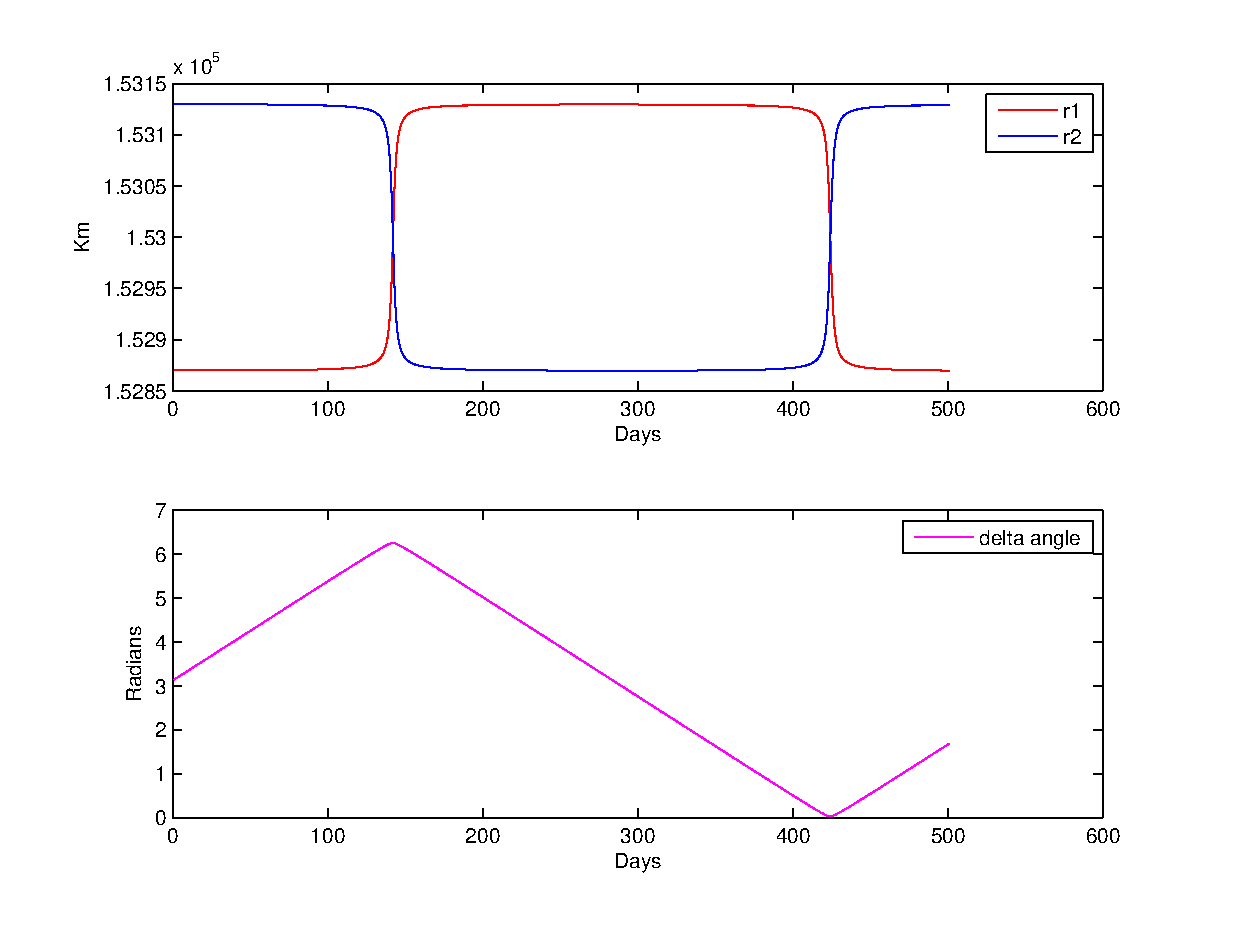
\includegraphics[width=1\textwidth]{./graphics/subplot.eps}
\caption[tekst i indholdsfortegnelsen]{The upper plot depicts the moons's distance to Saturn $r_1$ and $r_2$ as a function of time. The lower plot depicts the difference in the moons's angle $\theta_1$ and $\theta_2$.}
\label{fig:}
\end{figure}

\subsection{Precision of the results}
The local error at each iteration is set in $atol = 10^{-3}$ and $rtol = 0$. The \texttt{StepperStoerm<>} method in NR LIB uses the adaptive step size approach, meaning that the method will adapt the stepsize to have a smaller local error than $10^{-3}$.
When Output out(-1) is set the method outputs the steps that it uses to obtain a smaller local error than specified. \\
out.count gives the steps used by the method. In this exercise with $atol = 10^{-3}$, $rtol = 0$, $x1=0.0$ and $x2=500.0$ it gives 4166 steps.\\
The maximum global error at the last point must therefore be \\
$4166 \cdot 10^{-3} = 4.166  [km]$.
